\documentclass[parskip=full]{scrartcl}

\pdfoutput=1

\title{Improving Imbalanced Learning in Land Cover Classification \\ 
	\LARGE{A Heuristic Oversampling Method Based on K-Means and SMOTE}}
\author{
	Georgios Douzas\(^{1}\), Fernando Bacao\(^{1*}\), Joao Fonseca\(^{1}\)
	\\
	\small{\(^{1}\)NOVA Information Management School, Universidade Nova de Lisboa}
	\\
	\small{*Corresponding Author}
	\\
	\\
	\small{Postal Address: NOVA Information Management School, Campus de Campolide, 1070-312 Lisboa, Portugal}
	\\
	\small{Telephone: +351 21 382 8610}
}

\usepackage{breakcites}
\usepackage{float}
\usepackage{graphicx}
\usepackage{geometry}
\geometry{
	a4paper,
	total={170mm,257mm},
	left=18mm,
	right=18mm,
	top=8mm,
}
\usepackage{amsmath}
\newcommand{\inlineeqnum}{\refstepcounter{equation}~~\mbox{(\theequation)}}
\usepackage{enumitem}
\usepackage[ruled,vlined]{algorithm2e}
\usepackage{booktabs}
\usepackage{pgfplotstable}
\pgfplotsset{compat=1.14}
\usepackage{longtable}
\usepackage{tabu}
\usepackage{hyperref}
\date{}

\begin{document}

\maketitle

\begin{abstract}
	TODO TODO TODO TODO TODO TODO TODO TODO TODO TODO TODO TODO TODO TODO TODO TODO
	TODO TODO TODO TODO TODO TODO TODO TODO TODO TODO TODO TODO TODO TODO TODO TODO
	TODO TODO TODO TODO TODO TODO TODO TODO TODO TODO TODO TODO TODO TODO TODO TODO
	TODO TODO TODO TODO TODO TODO TODO TODO TODO TODO TODO TODO TODO TODO TODO TODO
	TODO TODO TODO TODO TODO TODO TODO TODO TODO TODO TODO TODO TODO TODO TODO TODO
	TODO TODO TODO TODO TODO TODO TODO TODO TODO TODO TODO TODO TODO TODO TODO TODO
	TODO TODO TODO TODO TODO TODO TODO TODO TODO TODO TODO TODO TODO TODO TODO TODO
\end{abstract}

\section{Introduction}

% context

The increasing amount of remote sensing missions granted the access to dense
time series (TS) data at a global level and provides up-to-date, accurate land
cover information \cite{Drusch2012}. This information is often
materialized through Land Use/Land Cover (LULC) maps, which constitute an
essential asset for various purposes, such as land cover change detection,
urban planning, environmental monitoring and natural hazard assessment
\cite{Khatami2016}. However, the production of accurate, updated LULC maps
still pose a challenge within the remote sensing community
\cite{Wulder2018}. They can have either one of two sources:
Photo-interpreted by the human eye, or Automatic mapping using remotely sensed
data and a classification algorithm.

Although photo-interpreted LULC maps rely on human interaction and can be more
reliable, they are not without its drawbacks: they are not frequently updated,
their production is time and resource consuming, not suitable for operational
mapping over large areas and are prone to overlook rare or small-area classes,
due to factors such as the minimum mapping unit being used. Concurrently,
machine-learning (ML) approaches face different challenges:
\begin{enumerate}
	\item Mislabelled LULC patches. As mentioned, the usage of photo-interpreted training
	      data poses a threat to the quality of any LULC map produced with this strategy,
	      since factors such as the minimum mapping unit tend to cause the overlooking of
	      small-area LULC patches and generates noisy training data that may reduce the
	      prediction power of a classifier \cite{Pelletier2017}.
	\item High-dimensional datasets. Multi-spectral TS composites are high-dimensional,
	      which increases the complexity of the problem and creates a strain on
	      computational power \cite{Stromann2020}.
	\item Class separability. The production of an accurate LULC map can be hindered by
	      the existence of classes with similar spectral signatures, making these classes
	      difficult to distinguish \cite{Alonso-Sarria2019}.
	\item Existence of rare land cover classes. Due to the varying levels of area
	      coverage for each class, the acquisition of training datasets containing
	      balanced class frequencies is often unfeasible. This causes an asymmetry in
	      class distribution, where some classes are frequent in the training dataset,
	      while others have little expression \cite{Wang2019, Feng2019}.
\end{enumerate}

% problem definition

The latter challenge is known, in the machine learning community, as the
imbalanced learning problem \cite{Chawla2004}. It is defined as a skewed
distribution of observations found in a dataset among classes in both binary
and multi-class problems \cite{Abdi2016}. This asymmetry in class
distribution negatively impacts the performance of classifiers, especially in
multi-class problems. During the learning phase, classifiers are optimized to
best fit an objective function, being the most common overall accuracy. During
this phase, observations belonging to rare classes contribute less towards the
predictive power of the corresponding classes, consequently inducing a bias
towards majority classes, as depicted in figure \ref{fig:oversampling_decision_function}a.

Typical ML algorithms are designed to perform well on relatively balanced
datasets. Although, defining a decision boundary on imbalanced datasets is a
difficult task, since each class' importance is typically as high as its
relative number of observations within the training dataset. There are three
different types of approaches to deal with the class imbalance problem
\cite{Fernandez2013}:
\begin{enumerate}
	\item Cost-sensitive solutions. Introduces a cost matrix to the learning phase with
	      misclassification costs attributed to each class. Minority classes will have a
	      higher cost than majority classes, forcing the algorithm to be more flexible
	      and adapt better to predict minority classes.
	\item Algorithmic level solutions. Specific classifiers are modified to reinforce the
	      learning on minority classes. Consists on the creation or adaptation of
	      classifiers.
	\item Resampling solutions. Rebalances the dataset's class distribution by removing
	      majority class instances and/or generating artificial minority instances (see
	      Figure \ref{fig:oversampling_decision_function}). This is considered an external  approach, where
	      the intervention occurs before the learning phase, benefitting from versatility
	      and independency from the classifier used.
\end{enumerate}

Within resampling approaches there are three subgroups of approaches:
\begin{enumerate}
	\item Undersampling methods. They rebalance class distribution by removing instances
	      from the majority classes.
	\item Oversampling methods. Dataset is rebalanced by generating new artificial
	      instances belonging to the minority classes.
	\item Hybrid methods. Combination of both oversampling and undersampling, resulting
	      in the removal of instances in the majority classes and the generation of
	      artificial instances in the minority classes.
\end{enumerate}

\begin{figure}[H]
	\centering
	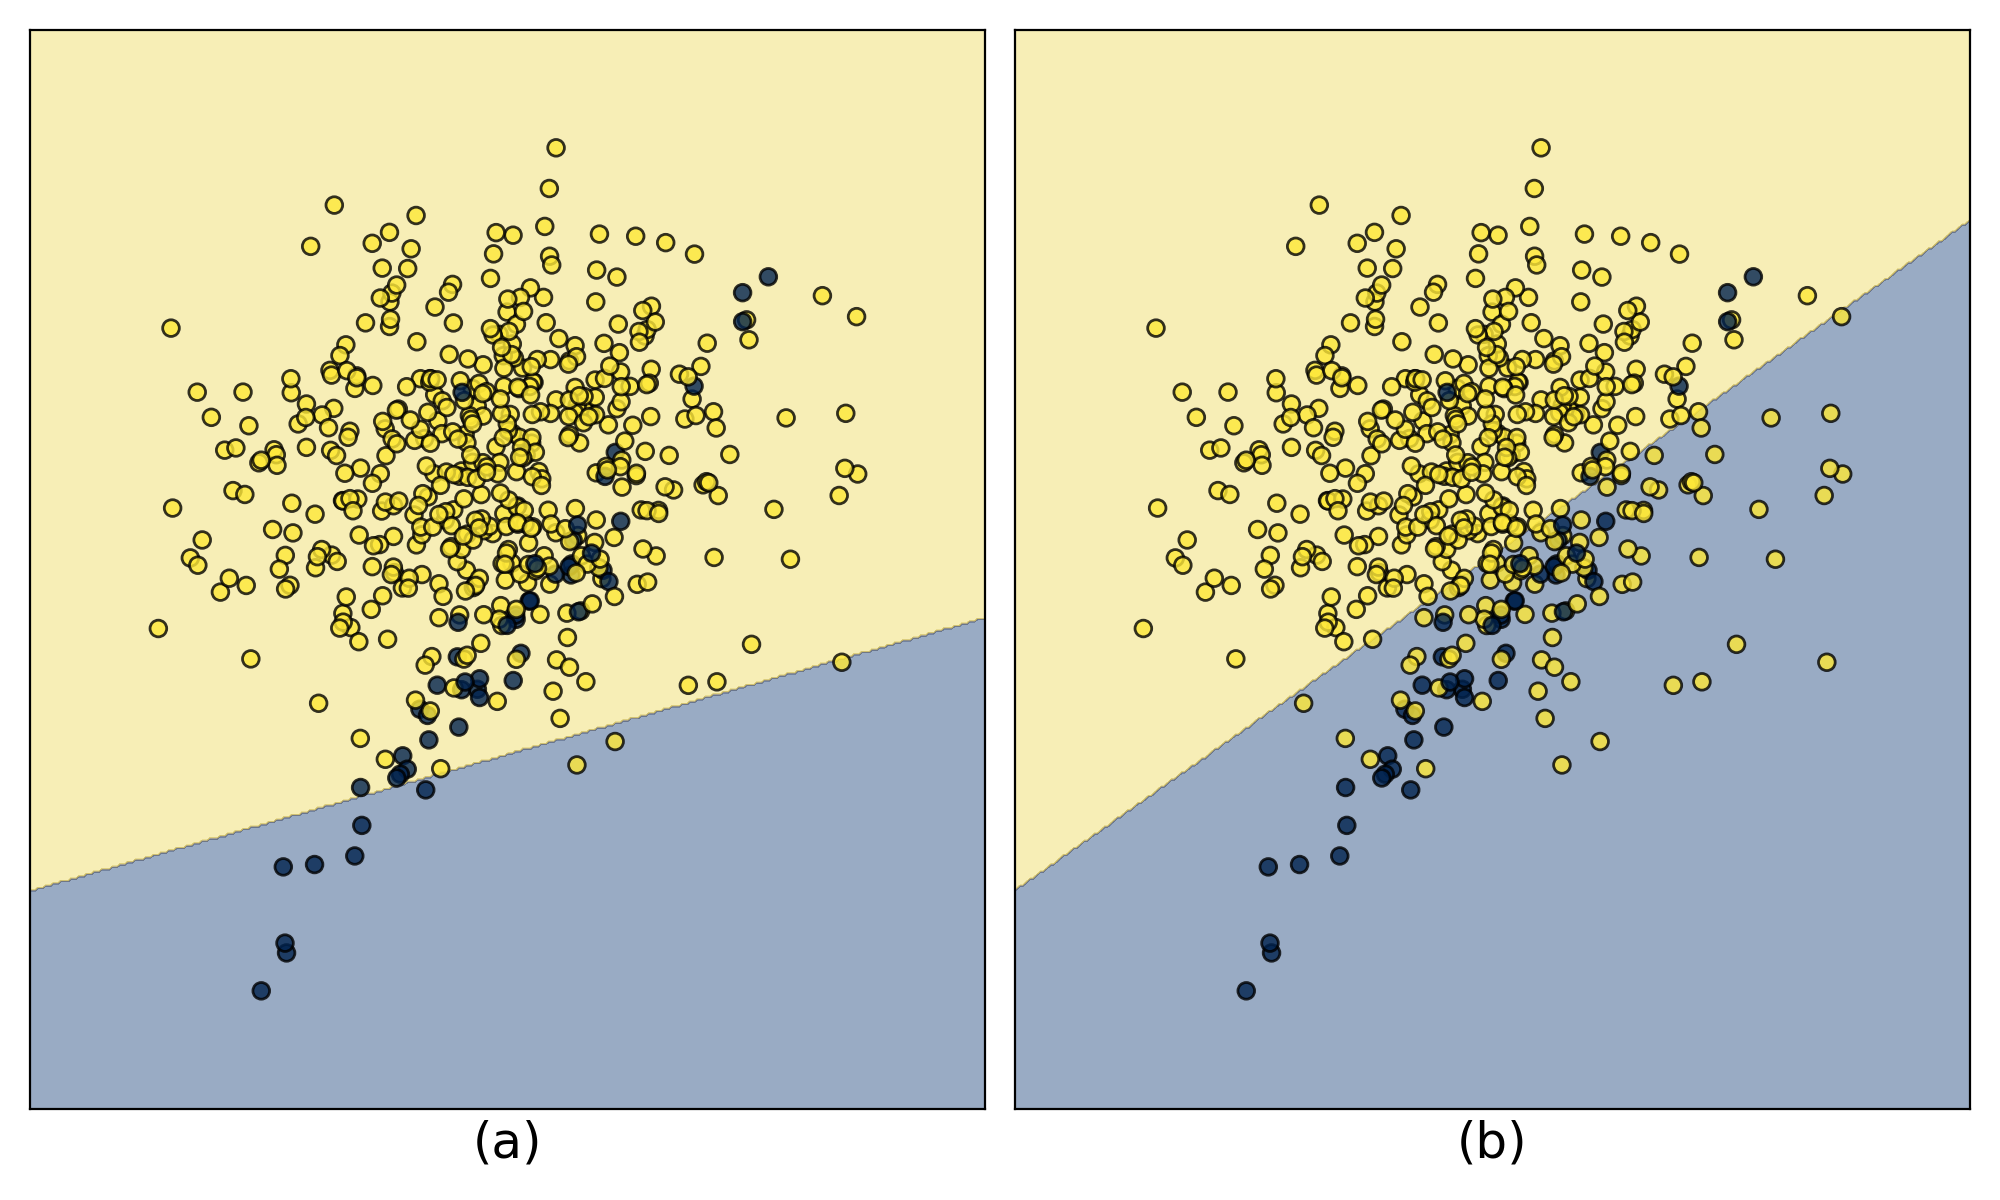
\includegraphics[width=.75\linewidth]{../analysis/oversampling_decision_function}
	\caption{Example of a linear Support Vector Machine's decision function (a) without
		resampling and (b) with resampling.}
	\label{fig:oversampling_decision_function}
\end{figure}

In this paper, we propose the K-means SMOTE (K-SMOTE) oversampler to address
the imbalanced learning problem for LULC classification and test its efficacy
on multiclass problems. To do so, we employ the both commonly used and
state-of-the-art oversamplers as benchmarking methods: Random oversampling,
SMOTE, ADASYN, Borderline-SMOTE and Geometric-SMOTE. As a baseline we also
present classification results without the employment of any resampling method.

% TODO: decide on the datasets

This paper is organized in \#\# sections: (TODO)

\section{Literature Review}

We divide our Literature Review analysis in related resampling methods and
applications

Even though existing approaches improve the predictive power of minority
classes, they also tend to generate noisy data points, which might harm the
quality of the final predictor

\bibliography{references}
\bibliographystyle{apalike}

\end{document}
